
\documentclass{exam}

\usepackage{graphicx}
\usepackage[fleqn]{amsmath}
\usepackage{unitsdef} 
\usepackage{cancel}
\usepackage{float}
\usepackage{mdwlist}
\usepackage{booktabs}
\usepackage{cancel}
\usepackage{polynom}
\usepackage{caption}
\usepackage{fullpage}
\usepackage{enumerate}

% \newcommand{\degree}{\ensuremath{^\circ}} 
\everymath{\displaystyle}

\newunit{\inch}{in}
\newunit{\foot}{ft}
\newunit{\cemtimeter}{cm}

% \begin{figure}[H]
%   \centering
%   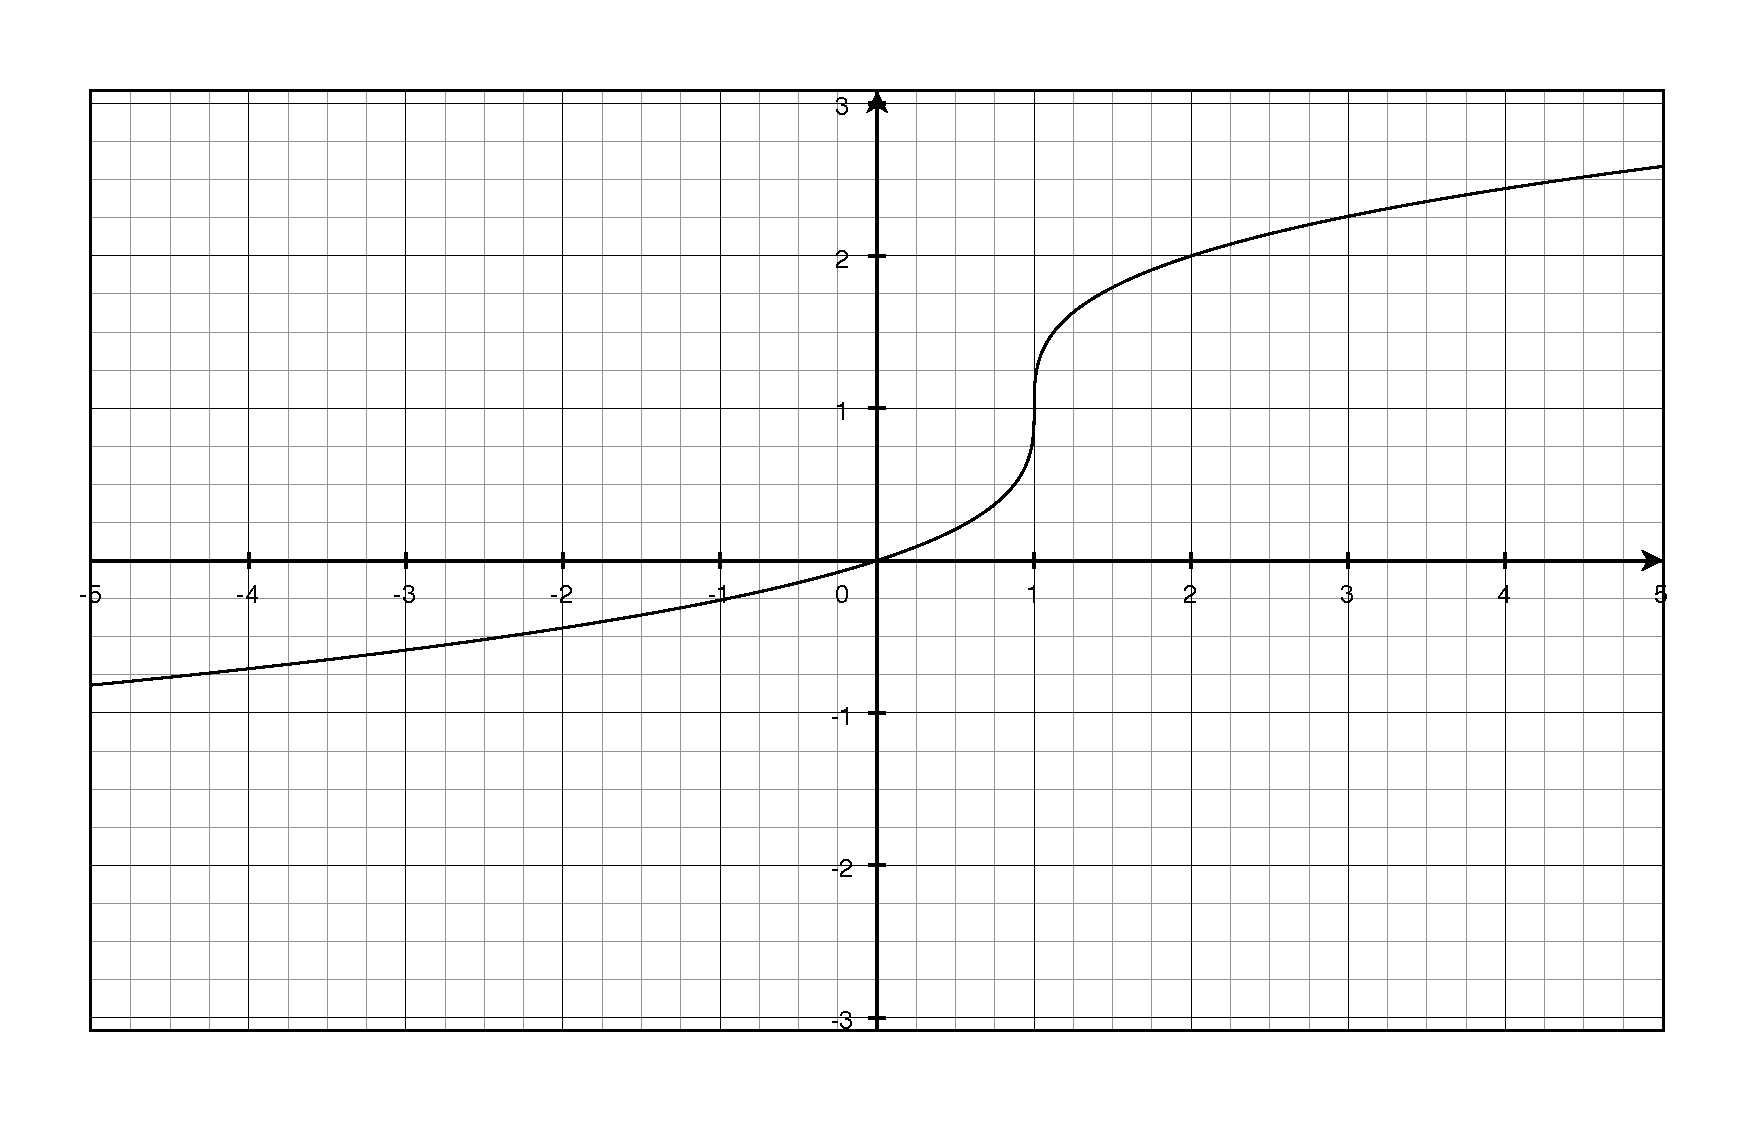
\includegraphics[scale=.3]{question7.eps}
%   \caption*{Question 7}
% \end{figure}

% \begin{tabular}{cc}
% \toprule
% period & amplitude \\
% \midrule
%   $\pi$ & $2$ \\
% \bottomrule
% \end{tabular}

\printanswers

\ifprintanswers 
\usepackage{2in1, lscape} 
\fi

\title{Math 263B \\ Homework Six}
\date{August 16, 2012}

\begin{document}

\maketitle

\ifprintanswers
\else
\section{Administrative}

Next week we'll review chapter 5 and the following week will be the chapter 5 exam.

\fi

\section{Homework}

\begin{itemize*}
  \item Read Section 5.7
  \item pp 290-292: 5-15, 20-25, 35-45, 51-55
\end{itemize*}

%% \ifprintanswers
%% \pagebreak
%% \fi

\section{Extra Credit}
page 291, problem 71

\begin{solution}
Since this is an even function, we can figure out the area for one half of the figure and then multiply by 2.  I worked
with the area to the right of the y axis.

The first thing to do is find an equation for the tangent line.  We know the slope is the derivative:
\begin{align*}
  y &= k \cos kx \\
  y' &= -k^2 \sin kx \\
\end{align*}

At the point we're interested in, the slope is:
\[
  y' \left( \frac{\pi}{2k} \right) = -k^2 \sin \left(k \cdot \frac{\pi}{2k} \right) = -k^2
\]

Now we know the slope, we can use the one point we know to find the y-intercept:
\begin{align*}
  y &= mx + b \\
  0 &= -k^2 \left(\frac{\pi}{2k} \right) + b \\
  b &= \frac{\pi k}{2} \\
\end{align*}

So the equation of the line is
\[
  y = -k^2x + \frac{\pi k}{2}
\]

The area under this line for the region is:
\begin{align*}
  \int_0^{\pi/2k} \left( -k^2x + \frac{\pi k}{2} \right) \, \mathrm{d}x = \frac{\pi^2}{8}
\end{align*}

The other area we need to find is the area under $y = k \cos kx$
\begin{align*}
  \int_0^{\pi/2k} k \cos kx \, \mathrm{d}x = \int_0^{\pi/2} \cos u \, \mathrm{d}u = 1
\end{align*}

So the area for this half of the figure is:
\[
  A_{half} = \frac{\pi^2}{8} - 1
\]

The total area is twice this:
\[
  A_{total} = 2 \left( \frac{\pi^2}{8} - 1 \right) = \frac{\pi^2}{4} - 2
\]


\end{solution}

\ifprintanswers

\section{Section 5.8}

\begin{description}

\item[5]
\begin{align*}
  u &= 3x + 2 \\
  dx &= \frac{du}{3} \\
\\
  \int \cos(3x + 2) \, \mathrm{d}x &= \frac{1}{3} \int \cos u \, \mathrm{d}u \\
  &= \frac{1}{3} \sin u + C \\
  &= \frac{1}{3} \sin(3x + 2) + C \\
\end{align*}

\item[6]
\begin{align*}
  u &= 2x - 4 \\
  dx &= \frac{du}{2} \\
\\
  \int \sin(2x - 4) \, \mathrm{d}x &= \frac{1}{2} \int \sin u \, \mathrm{d}u \\
  &= - \frac{1}{2} \cos u + C \\
  &= - \frac{1}{2} \cos (2x - 4) + C \\
\end{align*}

\item[7]
\begin{align*}
  u &= 6x - 7 \\
  dx &= \frac{du}{6} \\
\\
  \int \sin(6x - 7) \, \mathrm{d}x &= \frac{1}{6} \int \sin u \, \mathrm{d}u \\
  &= - \frac{1}{6} \cos u + C \\
  &= - \frac{1}{6} \cos (6x - 7) + C \\
\end{align*}

\item[8]
\begin{align*}
  u &= \pi v - \sqrt{7} \\
  dv &= \frac{du}{\pi} \\
\\
  \int \cos(\pi v - \sqrt{7} \, \mathrm{d}v &= \frac{1}{\pi} \int \cos u \, \mathrm{d}u \\
  &= \frac{1}{\pi} \sin u + C \\
  &= \frac{1}{\pi} \sin (\pi v - \sqrt{7}) + C \\
\end{align*}

\item[9]
\begin{align*}
  u &= x^2 + 4 \\
  du &= 2x \, dx \\
\\
  \int x (x^2 + 4)^{1/2} \, \mathrm{d}x &= \frac{1}{2} \int (x^2 + 4)^{1/2} 2x \, \mathrm{d}x \\
  &= \frac{1}{2} \int u^{1/2} \, \mathrm{d}u \\
  &= \frac{1}{3} u^{3/2} + C \\
  &= \frac{1}{3} (x^2 + 4)^{3/2} + C \\
\end{align*}

\item[10]
\begin{align*}
  u &= x^3 + 5 \\
  du &= 3x \, dx \\
\\
  \int x^2 (x^3 + 5)^9 \, \mathrm{d}x &= \frac{1}{3} \int (x^3 + 5)^9 \cdot 3x \, \mathrm{d}x \\
  &= \frac{1}{3} \int u^9 \, \mathrm{d}u \\
  &= \frac{1}{30} u^{10} + C \\
  &= \frac{1}{30} (x^3 + 5)^{10} + C \\
\end{align*}

\item[11]
\begin{align*}
  u &= x^2 + 3 \\
  du &= 2x \, dx \\
\\
  \int x (x^2 + 3)^{-12/7} \, \mathrm{d}x &= \frac{1}{2} \int (x^2 + 3)^{-12/7} \cdot 2x \, \mathrm{d}x \\
  &= \frac{1}{2} \int u^{-12/7} \, \mathrm{d}u \\
  &= - \frac{7}{10} u^{-5/7} + C \\
  &= - \frac{7}{10} (x^2 + 3)^{-5/7} + C \\
\end{align*}

\item[12]
\begin{align*}
  u &= \sqrt{3} v^2 + \pi \\
  du &= 2 \sqrt{3} v \, dv \\
\\
  \int v \left(\sqrt{3} v^2 + \pi\right)^{7/8} \, \mathrm{d}v &= \frac{1}{2 \sqrt{3}} \int \left(\sqrt{3} v^2 + \pi\right)^{7/8} \cdot 2 \sqrt{3} v \, \mathrm{d}v \\
  &= \frac{1}{2 \sqrt{3}} \int u^{7/8} \, \mathrm{d}u \\
  &= \frac{4}{15 \sqrt{3}} \cdot u^{15/8} + C \\
  &= \frac{4}{15 \sqrt{3}} \left(\sqrt{3} v^2 + \pi\right)^{15/8} + C \\
\end{align*}

\item[13]
\begin{align*}
  u &= x^2 + 4 \\
  du &= 2x \, dx \\
\\
  \int x \sin(x^2 + 4) \, \mathrm{d}x &= \frac{1}{2} \int \sin(x^2 + 4) \cdot 2x \, \mathrm{d}x \\
  &= \frac{1}{2} \int \sin u \, \mathrm{d}u \\
  &= - \frac{1}{2} \cos u + C \\
  &= - \frac{1}{2} \cos (x^2 + 4) + C \\
\end{align*}

\item[14]
\begin{align*}
  u &= x^3 + 5 \\
  du &= 3x^2 \, dx \\
\\
  \int x^2 \cos(x^3 + 5) \, \mathrm{d}x &= \frac{1}{3} \int \cos(x^3 + 5) \cdot 3x^2 \, \mathrm{d}x \\
  &= \frac{1}{3} \int \cos u \, \mathrm{d}u \\
  &= \frac{1}{3} \sin u + C \\
  &= \frac{1}{3} \sin (x^3 + 5) + C \\
\end{align*}

\item[15]
\begin{align*}
  u &= 6x^3 - 7 \\
  du &= 18x^2 \, dx \\
\\
  \int x^2 \sin(6x^3 - 7) \, \mathrm{d}x &= \frac{1}{18} \int \sin(6x^3 - 7) \cdot 18x^2 \, \mathrm{d}x \\
  &= \frac{1}{18} \int \sin u \, \mathrm{d}u \\
  &= -\frac{1}{18} \cos u + C \\
  &= -\frac{1}{18} \cos (6x^3 - 7) + C \\
\end{align*}

\item[20]
\begin{align*}
  u &= (7x^7 + \pi)^9 \\
  du &= 441 (7x^7 + \pi)^8 x^6 \, dx \\
\\
  \int x^6 (7x^7 + \pi)^8 &\sin[ (7x^7 + \pi)^9 ] \, \mathrm{d}x \\
  &= \frac{1}{441} \int \sin u \, \mathrm{d}u \\
  &= -\frac{1}{441} \cos u + C \\
  &= -\frac{1}{441} \cos [ (7x^7 + \pi)^9 ] + C \\
\end{align*}

\item[21]
\begin{align*}
  u &= \sin(x^2 + 4) \\
  du &= \cos(x^2 + 4) 2x \, dx \\
\\
  \int x \cos(x^2 + 4) &\sqrt{\sin{x^2 + 4}} \, \mathrm{d}x \\
  &= \frac{1}{2} \int \cos(x^2 + 4) \sqrt{\sin{x^2 + 4}} 2x \, \mathrm{d}x \\
  &= \frac{1}{2} \int u^{1/2} \, \mathrm{d}u \\
  &= \frac{1}{3} u^{3/2} + C \\
  &= \frac{1}{3} \sin^{3/2}(x^2 + 4) + C \\
\end{align*}

\item[22]
\begin{align*}
  u &= \cos(3x^7 + 9) \\
  du &= - \sin(3x^7 + 9) 21x^6 \, dx \\
\\
  \int x^6 \sin(3x^7 + 9) &\sqrt[3]{\cos(3^7 + 9)} \, \mathrm{d}x \\
  &= - \frac{1}{21} \int \sin(3x^7 + 9) \sqrt[3]{\cos(3^7 + 9)} \cdot 21x^6 \, \mathrm{d}x \\
  &= - \frac{1}{21} \int u^{1/3} \, \mathrm{d}u \\
  &= - \frac{1}{28} u^{4/3} + C \\
  &= - \frac{1}{28} \cos^{4/3}(3x^7 + 9) + C \\
\end{align*}

\item[23]
\begin{align*}
  u &= \cos(x^3 + 5) \\
  du &= - \sin(x^3 + 3) 3x^2 \, dx \\
\\
  \int x^2 \sin(x^3 + 5) & \left[ \cos(x^3 + 5) \right]^9 \, \mathrm{d}x \\
  &= - \frac{1}{3} \int \sin(x^3 + 5) \left[ \cos(x^3 + 5) \right]^9 3x^2 \, \mathrm{d}x \\
  &= -\frac{1}{3} \int u^9 \, \mathrm{d}u \\
  &= - \frac{1}{30} u^{10} + C \\
  &= - \frac{1}{30} \cos^{10}(x^3 + 5) + C \\
\end{align*}

\item[24]
\begin{align*}
  u &= \tan(x^{-3} + 1) \\
  du &= - \sec^2(x^{-3} + 1) 3x^{-4} \, dx \\
\\
  \int x^{-4} &\sec^2(x^{-3} + 1) \left[ \tan(x^{-3} + 1) \right]^{1/5} \, \mathrm{d}x \\
  &= - \frac{1}{3} \int 3x^{-4} \sec^2(x^{-3} + 1) \left[ \tan(x^{-3} + 1) \right]^{1/5} \, \mathrm{d}x \\
  &= - \frac{1}{3} \int u^{1/5} \, \mathrm{d}u \\
  &= - \frac{5}{18} u^{6/5} + C \\
  &= - \frac{5}{18} \tan^{6/5}(x^{-3} + 1) + C \\
\end{align*}

\item[25]
For this one, you first have to figure out $D_x \sec^{1/2} x$:
\begin{align*}
  D_x \sec^{1/2} x &= D_x (\cos x)^{-1/2} \\
  &= - \frac{1}{2} (\cos x)^{-3/2} (- \sin x) \\
  &= \frac{1}{2} \frac{\sin x}{\cos x} (\cos x)^{-1/2} \\
  &= \frac{1}{2} \tan x \sec^{1/2} x
\end{align*}

Now we're ready to solve the original problem:
\begin{align*}
  u &= \sec^{1/2}(x^2 + 2x) \\
  \frac{du}{dx} &= \frac{1}{2} \tan(x^2 + 2x) \sec^{1/2}(x^2 + 2x)(2x + 2) \\
  du &= \sec^{1/2}(x^2 + 2x)(x + 1) \tan(x^2 + 2x) \, dx \\
\\
  \int \sec^{1/2} & (x^2 + 2x)(x + 1) \tan(x^2 + 2x) \, \mathrm{d}x \\
  &= \int \, \mathrm{d}u \\
  &= u + C \\
  &= \sec^{1/2}(x^2 + 2x) + C \\
\end{align*}

\item[35]
\begin{align*}
  u &= x^2 + 4x + 1 \\
  du &= 2 (x + 2) \, dx \\
  u(0) &= 1 \\
  u(1) &= 6 \\
\\
  \int_0^1 & (x^2 + 4x + 1)^{-2} (x + 2) \, \mathrm{d}x \\
  &= \frac{1}{2} \int_0^1 (x^2 + 4x + 1)^{-2} \cdot 2 (x + 2) \, \mathrm{d}x \\
  &= \frac{1}{2} \int_1^6 u^{-2} \, \mathrm{d}x \\
  &= -\frac{1}{2u} \bigg|_1^6 \\
  &= \frac{5}{12} \\
\end{align*}

\item[36]
\begin{align*}
  u &= 9 - x^3 \\
  du &= -3x^2 \, dx \\
  u(0) &= 9 \\
  u(2) &= 1 \\
\\
  \int_0^2 & x^2 (9 - x^2)^{-3/2} \, \mathrm{d}x \\
  &= -\frac{1}{3} \int_0^2 (-3 x^2) (9 - x^2)^{-3/2} \, \mathrm{d}x \\
  &= -\frac{1}{3} \int_9^1 u^{-3/2} \, \mathrm{d}u \\
  &= \frac{4}{9} \\
\end{align*}

\item[37]
\begin{align*}
  u &= \sin \theta \\
  du &= \cos \theta \, d\theta \\
  u(0) &= 0 \\
  u(\pi/6) &= \frac{1}{2} \\
\\
  \int_0^{\pi/6} \sin^3 \theta \cos \theta\, \mathrm{d}\theta &= \int_0^{1/2} u^3 \, \mathrm{d}u \\
  &= \frac{1}{64} \\
\end{align*}

\item[38]
\begin{align*}
  u &= \cos \theta \\
  du &= - \sin \theta \, d\theta \\
  u(0) &= 1 \\
  u(\pi/6) &= \frac{\sqrt{3}}{2} \\
\\
  \int_0^{\pi/6} \cos^{-3} \theta \sin \theta\, \mathrm{d}\theta &= - \int_1^{\sqrt{3}/2} u^{-3} \, \mathrm{d}u \\
  &= - \frac{1}{6} \\
\end{align*}

\item[39]
\begin{align*}
  u &= 3x - 3 \\
  du &= 3 \, dx \\
  u(0) &= -3 \\
  u(1) &= 0 \\
\\
  \int_0^1 \cos(3x - 3) \, \mathrm{d}x &= \frac{1}{3} \int_{-3}^{0} \cos u \, \mathrm{d}u \\
  &= \frac{\sin u}{3} \bigg|_{-3}^{0} \\
  &= \frac{\sin 3}{3} \\
\end{align*}

\item[40]
\begin{align*}
  u &= 2 \pi x \\
  du &= 2 \pi \, dx \\
  u(0) &= 0 \\
  u(1/2) &= \pi \\
\\
  \int_0^{1/2} \sin(2 \pi x) \, \mathrm{d}x &= \frac{1}{2 \pi} \int_0^{\pi} u \, \mathrm{d}u \\
  &= \frac{1}{\pi} \\
\end{align*}

\item[41]
\begin{align*}
  u &= \pi x^2 \\
  du &= 2 \pi x \, dx \\
  u(0) &= 0 \\
  u(1) &= \pi \\
\\
  \int_0^{1} x \sin(\pi x^2) \, \mathrm{d}x &= \frac{1}{2 \pi} \int_0^{\pi} \sin u \, \mathrm{d}u \\
  &= \frac{- \cos u}{2 \pi} \bigg|_0^{\pi} \\
  &= \frac{1}{\pi} \\
\end{align*}

\item[42]
\begin{align*}
  u &= 2 x^5 \\
  du &= 10 x^4 \\
  u(0) &= 0 \\
  u(\pi) &= 2 \pi^5 \\
\\
  \int_0^{1} x^4 \cos(2 x^5) \, \mathrm{d}x &= \frac{1}{10} \int_0^{2 \pi^5} \cos u \, \mathrm{d}u \\
  &= \frac{\sin(2 \pi^5)}{10} \\
\end{align*}

\item[43]
\begin{align*}
  u &= 2x \\
  du &= 2 \, dx \\
  u(0) &= 0 \\
  u(\pi/4) &= \frac{\pi}{2} \\
\\
  \int_0^{\pi/4} (\cos 2x + \sin 2x) \, \mathrm{d}x &= \frac{1}{2} \int_0^{\pi/2} (\cos u + \sin u) \, \mathrm{d}u \\
  &= 1 \\
\end{align*}

\item[44]
\begin{align*}
  \int_{-\pi/2}^{\pi/2} (\cos 3x &+ \sin 5x) \, \mathrm{d}x \\
  &= \int_{-\pi/2}^{\pi/2} \cos 3x \, \mathrm{d}x + \int_{-\pi/2}^{\pi/2} \sin 5x \, \mathrm{d}x \\
  &= \frac{1}{3} \int_{-3\pi/2}^{3\pi/2} \cos u \, \mathrm{d}u + \frac{1}{5} \int_{-5\pi/2}^{5 \pi/2} \sin u \, \mathrm{d}u \\
  &= - \frac{2}{3} \\
\end{align*}

\item[45]
\begin{align*}
  u &= \cos x \\
  du &= \sin x \, dx \\
  u(0) &= 1 \\
  u(\pi/2) &= 0 \\
\\
  \int_0^{\pi/2} \sin x \sin(\cos x) \, \mathrm{d}x &= \int_1^0 \sin u \, \mathrm{d}u \
  &= \cos 0 - \cos 1 \\
  &= 1 - \cos 1 \\
  &\approx 0.4597 \\
\end{align*}

\item[51]
$\sin$ is odd, so
\[
  \int_{-\pi}^{\pi} \sin x \, \mathrm{d}x = 0
\]

\begin{align*}
  \int_{-\pi}^{\pi} (\sin x +  \cos x) \, \mathrm{d}x &= \int_{-\pi}^{\pi} \sin x \, \mathrm{d}x + \int_{-\pi}^{\pi} \cos x \, \mathrm{d}x  \\
  &= 0 + \int_{-\pi}^{\pi} \cos x \, \mathrm{d}x \\
  &= \sin x \bigg|_{-\pi}^{\pi} \\
  &= 0 \\
\end{align*}

\item[52]
\[
  f(-x) = \frac{(-x)^3}{(1 + x^2)^4} = - \frac{(x)^3}{(1 + x^2)^4} = - f(x)
\]

Since this is an odd function, the integral is zero.

\item[53]
\[
  f(-x) = \frac{\sin(-x)}{1 + \cos(-x)} = - \frac{\sin(x)}{1 + \cos(x)} = - f(x)
\]
Since this is an odd function, the integral is zero.

\item[54]
\begin{align*}
  \int_{-\sqrt[3]{\pi}}^{-\sqrt[3]{\pi}} x^2 \cos x^3 \, \mathrm{d}x &= 2 \int_0^{-\sqrt[3]{\pi}} x^2 \cos x^3 \, \mathrm{d}x \\
  &= \frac{2}{3} \int_0^{\pi} \cos u \, \mathrm{d}u \\
  &= \frac{2}{3} \sin u \bigg|_0^{\pi} \\
  &= 0 \\
\end{align*}

\item[55]
$f(x) = \sin x \cos x$ comes up in this problem, and this is an odd function:
\[
  f(-x) = \sin(-x) \cos(-x) = - \sin x \cos x = - f(x)
\]

so:
\[
  \int_{-\pi}^{\pi} \sin x \cos x \, \mathrm{d}x = 0
\]

If you expand the original problem, you get:
\begin{align*}
  \int_{-\pi}^{\pi} (\sin x + \cos x) \, \mathrm{d}x &= \int_{-\pi}^{\pi} (\sin^2 x + \cos^2 x + 2 \sin x \cos x) \, \mathrm{d}x \\
  &= \int_{-\pi}^{\pi} (1 + 2 \sin x \cos x) \, \mathrm{d}x \\
  &= \int_{-\pi}^{\pi} \, \mathrm{d}x + 2 \int_{-\pi}^{\pi} \sin x \cos x \, \mathrm{d}x \\
  &= 2 \pi + 2 \int_{-\pi}^{\pi} \sin x \cos x \, \mathrm{d}x \\
  &= 2 \pi \\
\end{align*}

\end{description}

\else

\vspace{8 cm}

%% The most effective way to restrict democracy is to transfer decision-making from the public arena to unaccountable
%% institutions: kings and princes, priestly castes, military juntas, party dictatorships, or modern corporations.

%% \hspace{0.5 cm} --Noam Chomsky

%% {\em Some writers have so confounded society with government, as to leave little or no distinction between them; whereas
%%   they are not only different, but have different origins. Society is produced by our wants, and government by our
%%   wickedness; the former promotes our happiness POSITIVELY by uniting our affections, the latter NEGATIVELY by
%%   restraining our vices. The one encourages intercourse, the other creates distinctions. The first a patron, the last a
%%   punisher.} --Thomas Paine

{\em I build no system. I ask an end to privilege, the abolition of slavery, equality of rights, and the reign of
law. Justice, nothing else; that is the alpha and omega of my argument: to others I leave the business of governing the
world.}

\vspace{.2 cm}

\hspace{1 cm} --Pierre-Joseph Proudhon

\fi

\end{document}

